\documentclass{book}
\usepackage[a4paper,top=2.5cm,bottom=2.5cm,left=2.5cm,right=2.5cm]{geometry}
\usepackage{makeidx}
\usepackage{natbib}
\usepackage{graphicx}
\usepackage{multicol}
\usepackage{float}
\usepackage{listings}
\usepackage{color}
\usepackage{ifthen}
\usepackage[table]{xcolor}
\usepackage{textcomp}
\usepackage{alltt}
\usepackage{ifpdf}
\ifpdf
\usepackage[pdftex,
            pagebackref=true,
            colorlinks=true,
            linkcolor=blue,
            unicode
           ]{hyperref}
\else
\usepackage[ps2pdf,
            pagebackref=true,
            colorlinks=true,
            linkcolor=blue,
            unicode
           ]{hyperref}
\usepackage{pspicture}
\fi
\usepackage[utf8]{inputenc}
\usepackage{mathptmx}
\usepackage[scaled=.90]{helvet}
\usepackage{courier}
\usepackage{sectsty}
\usepackage{amssymb}
\usepackage[titles]{tocloft}
\usepackage{doxygen}
\lstset{language=C++,inputencoding=utf8,basicstyle=\footnotesize,breaklines=true,breakatwhitespace=true,tabsize=4,numbers=left }
\makeindex
\setcounter{tocdepth}{3}
\renewcommand{\footrulewidth}{0.4pt}
\renewcommand{\familydefault}{\sfdefault}
\hfuzz=15pt
\setlength{\emergencystretch}{15pt}
\hbadness=750
\tolerance=750
\begin{document}
\hypersetup{pageanchor=false,citecolor=blue}
\begin{titlepage}
\vspace*{7cm}
\begin{center}
{\Large F\-S\-M\-L++ }\\
\vspace*{1cm}
{\large Generated by Doxygen 1.8.3.1}\\
\vspace*{0.5cm}
{\small Tue Jan 7 2014 20:19:52}\\
\end{center}
\end{titlepage}
\clearemptydoublepage
\pagenumbering{roman}
\tableofcontents
\clearemptydoublepage
\pagenumbering{arabic}
\hypersetup{pageanchor=true,citecolor=blue}
\chapter{F\-S\-M\-L++}
\label{md_README}
\hypertarget{md_README}{}
F\-S\-M\-L implementation using C++ -- see \href{https://github.com/slebok/slepro/tree/master/languages/fsml}{\tt https\-://github.\-com/slebok/slepro/tree/master/languages/fsml}

\subsection*{Requirements }

This program requires a compiler that supports the C++11 standard.

It also depends on Boost, which is provided in the lib folder to be linked statically. There's no need to build Boost, as only header files are used.

For unit testing, Google's gtest library and pthread are required.

Finally, since the program generates La\-Te\-X and Dot code, you will need appropriate programs for compiling them, e.\-g. pdf\-Te\-X and Graphviz

\subsection*{Build }

There is a Makefile for gcc provided, which will place compiled binaries into a folder called bin.

Use {\ttfamily make debug} or {\ttfamily make release} to build a debug or fully-\/optimized executable. The binaries will be called {\ttfamily fsmlpp\-\_\-debug} and {\ttfamily fsmlpp} respectively.

Use {\ttfamily make simulation} to build the sample interactive simulation. If you have Google's gtest unit testing library and pthread installed. The resulting binary will be called {\ttfamily fsmlpp\-\_\-simulation}.

Use {\ttfamily make test} to build the unit test, the required libraries will be attempted to be linked via {\ttfamily -\/lgtest -\/lpthread} The resulting binary will be called {\ttfamily fsmlpp\-\_\-test}.

{\ttfamily make} by itself will build all targets.

\subsection*{Bash Script }

There is a bash script called {\ttfamily buildnrun.\-sh} provided. It will make the release build, generate C++, La\-Te\-X and Dot code for the Sample.\-Fsml, and finally run {\ttfamily pdflatex} and {\ttfamily graphviz} to yield two different P\-D\-F files.

\subsection*{Run F\-S\-M\-L++ }

The syntax for running the program is {\ttfamily fsmlpp S\-O\-U\-R\-C\-E}, where S\-O\-U\-R\-C\-E is the path to a file containing F\-S\-M\-L code.

Note that the program will look for the template files in the present working directory, so run it from the project's root directory.

The program will attempt to load the given file, parse the code inside, validate it and then generate a C++ header file, La\-Te\-X file and Dot file with an appropriate name. If any of the steps fail, an appropriate error is thrown.

\subsection*{Run Test }

Execute the compiled {\ttfamily fsmlpp\-\_\-test} from the project's root directory so it can find all files. No special output means that the expected errors or lack thereof occurred. Otherwise, there will be a message about each failed test.

\subsection*{Run Simulation }

To run the simulation, just execute the compiled {\ttfamily fsmlpp\-\_\-simulation} and enjoy the interactive simulation experience. 
\chapter{Hierarchical Index}
\section{Class Hierarchy}
This inheritance list is sorted roughly, but not completely, alphabetically\-:\begin{DoxyCompactList}
\item \contentsline{section}{fsml\-:\-:Action}{\pageref{classfsml_1_1Action}}{}
\item \contentsline{section}{fsml\-:\-:Ast\-Machine}{\pageref{structfsml_1_1AstMachine}}{}
\item \contentsline{section}{fsml\-:\-:Ast\-State}{\pageref{structfsml_1_1AstState}}{}
\item \contentsline{section}{fsml\-:\-:Ast\-Step}{\pageref{structfsml_1_1AstStep}}{}
\item \contentsline{section}{fsml\-:\-:Flat\-Machine}{\pageref{structfsml_1_1FlatMachine}}{}
\item \contentsline{section}{fsml\-:\-:Flat\-Step}{\pageref{structfsml_1_1FlatStep}}{}
\item \contentsline{section}{fsml\-:\-:Machine}{\pageref{classfsml_1_1Machine}}{}
\item runtime\-\_\-error\begin{DoxyCompactList}
\item \contentsline{section}{fsml\-:\-:Deterministic\-Exception}{\pageref{structfsml_1_1DeterministicException}}{}
\item \contentsline{section}{fsml\-:\-:File\-Read\-Exception}{\pageref{structfsml_1_1FileReadException}}{}
\item \contentsline{section}{fsml\-:\-:File\-Write\-Exception}{\pageref{structfsml_1_1FileWriteException}}{}
\item \contentsline{section}{fsml\-:\-:Initial\-State\-Exception}{\pageref{structfsml_1_1InitialStateException}}{}
\item \contentsline{section}{fsml\-:\-:Invalid\-Input\-Exception}{\pageref{structfsml_1_1InvalidInputException}}{}
\item \contentsline{section}{fsml\-:\-:Parser\-Exception}{\pageref{structfsml_1_1ParserException}}{}
\item \contentsline{section}{fsml\-:\-:Reachable\-Exception}{\pageref{structfsml_1_1ReachableException}}{}
\item \contentsline{section}{fsml\-:\-:Resolvable\-Exception}{\pageref{structfsml_1_1ResolvableException}}{}
\item \contentsline{section}{fsml\-:\-:Unique\-Exception}{\pageref{structfsml_1_1UniqueException}}{}
\end{DoxyCompactList}
\item \contentsline{section}{fsml\-:\-:State}{\pageref{classfsml_1_1State}}{}
\item \contentsline{section}{fsml\-:\-:Step}{\pageref{classfsml_1_1Step}}{}
\end{DoxyCompactList}

\chapter{Class Index}
\section{Class List}
Here are the classes, structs, unions and interfaces with brief descriptions\-:\begin{DoxyCompactList}
\item\contentsline{section}{\hyperlink{classfsml_1_1Action}{fsml\-::\-Action} \\*Represents a transition action }{\pageref{classfsml_1_1Action}}{}
\item\contentsline{section}{\hyperlink{structfsml_1_1AstMachine}{fsml\-::\-Ast\-Machine} \\*Abstract syntax tree representation of a state machine }{\pageref{structfsml_1_1AstMachine}}{}
\item\contentsline{section}{\hyperlink{structfsml_1_1AstState}{fsml\-::\-Ast\-State} \\*Abstract syntax tree representation of a state }{\pageref{structfsml_1_1AstState}}{}
\item\contentsline{section}{\hyperlink{structfsml_1_1AstStep}{fsml\-::\-Ast\-Step} \\*Abstract syntax tree representation of a transition }{\pageref{structfsml_1_1AstStep}}{}
\item\contentsline{section}{\hyperlink{structfsml_1_1DeterministicException}{fsml\-::\-Deterministic\-Exception} \\*Exception thrown if input in \hyperlink{classfsml_1_1State}{State} is not deterministic }{\pageref{structfsml_1_1DeterministicException}}{}
\item\contentsline{section}{\hyperlink{structfsml_1_1FileReadException}{fsml\-::\-File\-Read\-Exception} \\*Exception thrown if an error occurs reading from a file }{\pageref{structfsml_1_1FileReadException}}{}
\item\contentsline{section}{\hyperlink{structfsml_1_1FileWriteException}{fsml\-::\-File\-Write\-Exception} \\*Exception thrown if an error occurs writing to a file }{\pageref{structfsml_1_1FileWriteException}}{}
\item\contentsline{section}{\hyperlink{structfsml_1_1FlatMachine}{fsml\-::\-Flat\-Machine} \\*Flat representation of the abstract syntax tree }{\pageref{structfsml_1_1FlatMachine}}{}
\item\contentsline{section}{\hyperlink{structfsml_1_1FlatStep}{fsml\-::\-Flat\-Step} \\*Flat representation of a transition }{\pageref{structfsml_1_1FlatStep}}{}
\item\contentsline{section}{\hyperlink{structfsml_1_1InitialStateException}{fsml\-::\-Initial\-State\-Exception} \\*Exception thrown if a \hyperlink{classfsml_1_1Machine}{Machine} constructs with more or less than one initial state }{\pageref{structfsml_1_1InitialStateException}}{}
\item\contentsline{section}{\hyperlink{structfsml_1_1InvalidInputException}{fsml\-::\-Invalid\-Input\-Exception} \\*Exception thrown if an invalid input is fed into a \hyperlink{classfsml_1_1Machine}{Machine} }{\pageref{structfsml_1_1InvalidInputException}}{}
\item\contentsline{section}{\hyperlink{classfsml_1_1Machine}{fsml\-::\-Machine} \\*Represents a simulatable final state machine }{\pageref{classfsml_1_1Machine}}{}
\item\contentsline{section}{\hyperlink{structfsml_1_1ParserException}{fsml\-::\-Parser\-Exception} \\*Exception thrown if parsing fails }{\pageref{structfsml_1_1ParserException}}{}
\item\contentsline{section}{\hyperlink{structfsml_1_1ReachableException}{fsml\-::\-Reachable\-Exception} \\*Exception thrown if not all States in a \hyperlink{classfsml_1_1Machine}{Machine} are reachable }{\pageref{structfsml_1_1ReachableException}}{}
\item\contentsline{section}{\hyperlink{structfsml_1_1ResolvableException}{fsml\-::\-Resolvable\-Exception} \\*Exception thrown if the target of a \hyperlink{classfsml_1_1Step}{Step} is not resolvable }{\pageref{structfsml_1_1ResolvableException}}{}
\item\contentsline{section}{\hyperlink{classfsml_1_1State}{fsml\-::\-State} \\*Represents a \hyperlink{classfsml_1_1Machine}{Machine}'s state }{\pageref{classfsml_1_1State}}{}
\item\contentsline{section}{\hyperlink{classfsml_1_1Step}{fsml\-::\-Step} \\*Represents a \hyperlink{classfsml_1_1State}{State}'s transition }{\pageref{classfsml_1_1Step}}{}
\item\contentsline{section}{\hyperlink{structfsml_1_1UniqueException}{fsml\-::\-Unique\-Exception} \\*Exception thrown if a \hyperlink{classfsml_1_1State}{State}'s name in a \hyperlink{classfsml_1_1Machine}{Machine} is not unique }{\pageref{structfsml_1_1UniqueException}}{}
\end{DoxyCompactList}

\chapter{Class Documentation}
\hypertarget{classfsml_1_1Action}{\section{fsml\-:\-:Action Class Reference}
\label{classfsml_1_1Action}\index{fsml\-::\-Action@{fsml\-::\-Action}}
}


Represents a transition action.  




{\ttfamily \#include $<$Action.\-hpp$>$}

\subsection*{Public Member Functions}
\begin{DoxyCompactItemize}
\item 
\hypertarget{classfsml_1_1Action_aa2434deec70591006e204eb7fb0e97d7}{{\bfseries Action} (const std\-::string \&\hyperlink{classfsml_1_1Action_ab5da63bc94cdd0b4110c87fd3e4ee271}{id})}\label{classfsml_1_1Action_aa2434deec70591006e204eb7fb0e97d7}

\item 
virtual const std\-::string \& \hyperlink{classfsml_1_1Action_ab158f49a59dea6cf40ba08210dcd09cc}{get\-Id} () const 
\item 
virtual void \hyperlink{classfsml_1_1Action_ac41cfae7343d8b96fbd204451bee840f}{register\-Function} (const Action\-Function \&f)
\begin{DoxyCompactList}\small\item\em Registers the given function. \end{DoxyCompactList}\item 
virtual void \hyperlink{classfsml_1_1Action_ae5b8ae5409ea58bed119bc860a803897}{invoke} () const 
\begin{DoxyCompactList}\small\item\em Invokes the previously registered function. \end{DoxyCompactList}\end{DoxyCompactItemize}
\subsection*{Protected Attributes}
\begin{DoxyCompactItemize}
\item 
\hypertarget{classfsml_1_1Action_ab5da63bc94cdd0b4110c87fd3e4ee271}{const std\-::string \hyperlink{classfsml_1_1Action_ab5da63bc94cdd0b4110c87fd3e4ee271}{id}}\label{classfsml_1_1Action_ab5da63bc94cdd0b4110c87fd3e4ee271}

\begin{DoxyCompactList}\small\item\em The name of this action. \end{DoxyCompactList}\item 
\hypertarget{classfsml_1_1Action_a40fbbd85f83fd1c0b5260584a24469ee}{Action\-Function \hyperlink{classfsml_1_1Action_a40fbbd85f83fd1c0b5260584a24469ee}{func}}\label{classfsml_1_1Action_a40fbbd85f83fd1c0b5260584a24469ee}

\begin{DoxyCompactList}\small\item\em The function. \end{DoxyCompactList}\end{DoxyCompactItemize}


\subsection{Detailed Description}
Represents a transition action. 



\subsection{Member Function Documentation}
\hypertarget{classfsml_1_1Action_ab158f49a59dea6cf40ba08210dcd09cc}{\index{fsml\-::\-Action@{fsml\-::\-Action}!get\-Id@{get\-Id}}
\index{get\-Id@{get\-Id}!fsml::Action@{fsml\-::\-Action}}
\subsubsection[{get\-Id}]{\setlength{\rightskip}{0pt plus 5cm}const string \& fsml\-::\-Action\-::get\-Id (
\begin{DoxyParamCaption}
{}
\end{DoxyParamCaption}
) const\hspace{0.3cm}{\ttfamily [virtual]}}}\label{classfsml_1_1Action_ab158f49a59dea6cf40ba08210dcd09cc}
\begin{DoxyReturn}{Returns}
The \hyperlink{classfsml_1_1Action}{Action}'s name 
\end{DoxyReturn}
\hypertarget{classfsml_1_1Action_ae5b8ae5409ea58bed119bc860a803897}{\index{fsml\-::\-Action@{fsml\-::\-Action}!invoke@{invoke}}
\index{invoke@{invoke}!fsml::Action@{fsml\-::\-Action}}
\subsubsection[{invoke}]{\setlength{\rightskip}{0pt plus 5cm}void fsml\-::\-Action\-::invoke (
\begin{DoxyParamCaption}
{}
\end{DoxyParamCaption}
) const\hspace{0.3cm}{\ttfamily [virtual]}}}\label{classfsml_1_1Action_ae5b8ae5409ea58bed119bc860a803897}


Invokes the previously registered function. 

\hypertarget{classfsml_1_1Action_ac41cfae7343d8b96fbd204451bee840f}{\index{fsml\-::\-Action@{fsml\-::\-Action}!register\-Function@{register\-Function}}
\index{register\-Function@{register\-Function}!fsml::Action@{fsml\-::\-Action}}
\subsubsection[{register\-Function}]{\setlength{\rightskip}{0pt plus 5cm}void fsml\-::\-Action\-::register\-Function (
\begin{DoxyParamCaption}
\item[{const Action\-Function \&}]{f}
\end{DoxyParamCaption}
)\hspace{0.3cm}{\ttfamily [virtual]}}}\label{classfsml_1_1Action_ac41cfae7343d8b96fbd204451bee840f}


Registers the given function. 


\begin{DoxyParams}{Parameters}
{\em f} & The function. \\
\hline
\end{DoxyParams}


The documentation for this class was generated from the following files\-:\begin{DoxyCompactItemize}
\item 
include/fsml/Action.\-hpp\item 
src/fsml/Action.\-cpp\end{DoxyCompactItemize}

\hypertarget{structfsml_1_1AstMachine}{\section{fsml\-:\-:Ast\-Machine Struct Reference}
\label{structfsml_1_1AstMachine}\index{fsml\-::\-Ast\-Machine@{fsml\-::\-Ast\-Machine}}
}


Abstract syntax tree representation of a state machine.  




{\ttfamily \#include $<$Parser.\-hpp$>$}

\subsection*{Public Attributes}
\begin{DoxyCompactItemize}
\item 
\hypertarget{structfsml_1_1AstMachine_a007b560f2e500f7f51c570f0316843e2}{std\-::vector$<$ \hyperlink{structfsml_1_1AstState}{Ast\-State} $>$ {\bfseries states}}\label{structfsml_1_1AstMachine_a007b560f2e500f7f51c570f0316843e2}

\end{DoxyCompactItemize}


\subsection{Detailed Description}
Abstract syntax tree representation of a state machine. 



The documentation for this struct was generated from the following file\-:\begin{DoxyCompactItemize}
\item 
include/fsml/Parser.\-hpp\end{DoxyCompactItemize}

\hypertarget{structfsml_1_1AstState}{\section{fsml\-:\-:Ast\-State Struct Reference}
\label{structfsml_1_1AstState}\index{fsml\-::\-Ast\-State@{fsml\-::\-Ast\-State}}
}


Abstract syntax tree representation of a state.  




{\ttfamily \#include $<$Ast.\-hpp$>$}

\subsection*{Public Attributes}
\begin{DoxyCompactItemize}
\item 
\hypertarget{structfsml_1_1AstState_a89a44c91811564d41c48343cf34560cd}{std\-::string {\bfseries initial}}\label{structfsml_1_1AstState_a89a44c91811564d41c48343cf34560cd}

\item 
\hypertarget{structfsml_1_1AstState_a3e7e96d12d2e17d8d35d313b232cb4f5}{std\-::string {\bfseries id}}\label{structfsml_1_1AstState_a3e7e96d12d2e17d8d35d313b232cb4f5}

\item 
\hypertarget{structfsml_1_1AstState_a39a00b99d02537f2b014556c203d9c36}{std\-::vector$<$ \hyperlink{structfsml_1_1AstStep}{Ast\-Step} $>$ {\bfseries steps}}\label{structfsml_1_1AstState_a39a00b99d02537f2b014556c203d9c36}

\end{DoxyCompactItemize}


\subsection{Detailed Description}
Abstract syntax tree representation of a state. 



The documentation for this struct was generated from the following file\-:\begin{DoxyCompactItemize}
\item 
include/fsml/Ast.\-hpp\end{DoxyCompactItemize}

\hypertarget{structfsml_1_1AstStep}{\section{fsml\-:\-:Ast\-Step Struct Reference}
\label{structfsml_1_1AstStep}\index{fsml\-::\-Ast\-Step@{fsml\-::\-Ast\-Step}}
}


Abstract syntax tree representation of a transition.  




{\ttfamily \#include $<$Parser.\-hpp$>$}

\subsection*{Public Attributes}
\begin{DoxyCompactItemize}
\item 
\hypertarget{structfsml_1_1AstStep_a2244e46f2cff2fa65fda13931a377356}{std\-::string {\bfseries input}}\label{structfsml_1_1AstStep_a2244e46f2cff2fa65fda13931a377356}

\item 
\hypertarget{structfsml_1_1AstStep_a308747ad3a3acc808f6c654ff1942e96}{std\-::string {\bfseries action}}\label{structfsml_1_1AstStep_a308747ad3a3acc808f6c654ff1942e96}

\item 
\hypertarget{structfsml_1_1AstStep_ac7eb1fb884326a326da14c054d3f7777}{std\-::string {\bfseries target}}\label{structfsml_1_1AstStep_ac7eb1fb884326a326da14c054d3f7777}

\end{DoxyCompactItemize}


\subsection{Detailed Description}
Abstract syntax tree representation of a transition. 



The documentation for this struct was generated from the following file\-:\begin{DoxyCompactItemize}
\item 
include/fsml/Parser.\-hpp\end{DoxyCompactItemize}

\hypertarget{structfsml_1_1DeterministicException}{\section{fsml\-:\-:Deterministic\-Exception Struct Reference}
\label{structfsml_1_1DeterministicException}\index{fsml\-::\-Deterministic\-Exception@{fsml\-::\-Deterministic\-Exception}}
}


Exception thrown if input in \hyperlink{classfsml_1_1State}{State} is not deterministic.  




{\ttfamily \#include $<$Exceptions.\-hpp$>$}

Inheritance diagram for fsml\-:\-:Deterministic\-Exception\-:\begin{figure}[H]
\begin{center}
\leavevmode
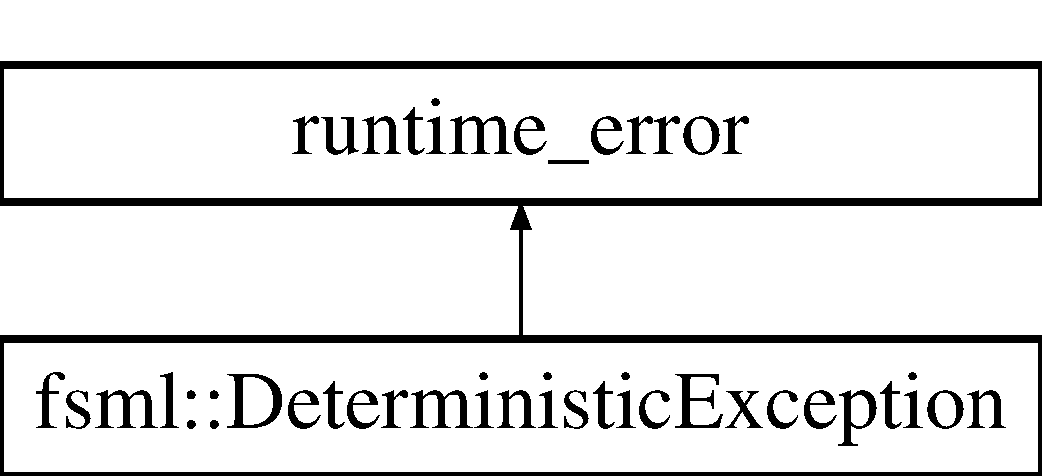
\includegraphics[height=2.000000cm]{structfsml_1_1DeterministicException}
\end{center}
\end{figure}
\subsection*{Public Member Functions}
\begin{DoxyCompactItemize}
\item 
\hypertarget{structfsml_1_1DeterministicException_ac8f4f6c7ee0d7cad65cd1f90ef506b71}{{\bfseries Deterministic\-Exception} (const std\-::string \&input, const std\-::string \&state)}\label{structfsml_1_1DeterministicException_ac8f4f6c7ee0d7cad65cd1f90ef506b71}

\end{DoxyCompactItemize}


\subsection{Detailed Description}
Exception thrown if input in \hyperlink{classfsml_1_1State}{State} is not deterministic. 



The documentation for this struct was generated from the following files\-:\begin{DoxyCompactItemize}
\item 
include/fsml/Exceptions.\-hpp\item 
src/fsml/Exceptions.\-cpp\end{DoxyCompactItemize}

\hypertarget{structfsml_1_1FileReadException}{\section{fsml\-:\-:File\-Read\-Exception Struct Reference}
\label{structfsml_1_1FileReadException}\index{fsml\-::\-File\-Read\-Exception@{fsml\-::\-File\-Read\-Exception}}
}


Exception thrown if an error occurs reading from a file.  




{\ttfamily \#include $<$Exceptions.\-hpp$>$}

Inheritance diagram for fsml\-:\-:File\-Read\-Exception\-:\begin{figure}[H]
\begin{center}
\leavevmode
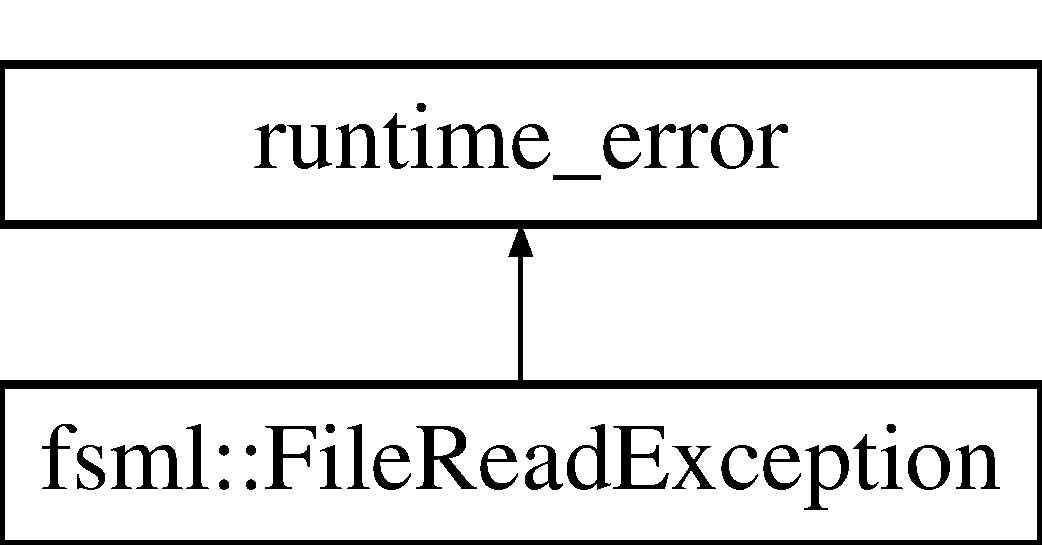
\includegraphics[height=2.000000cm]{structfsml_1_1FileReadException}
\end{center}
\end{figure}
\subsection*{Public Member Functions}
\begin{DoxyCompactItemize}
\item 
\hypertarget{structfsml_1_1FileReadException_a659fb09fec2fb56251b07ff27ddc1389}{{\bfseries File\-Read\-Exception} (const std\-::string \&file)}\label{structfsml_1_1FileReadException_a659fb09fec2fb56251b07ff27ddc1389}

\end{DoxyCompactItemize}


\subsection{Detailed Description}
Exception thrown if an error occurs reading from a file. 



The documentation for this struct was generated from the following files\-:\begin{DoxyCompactItemize}
\item 
include/fsml/Exceptions.\-hpp\item 
src/fsml/Exceptions.\-cpp\end{DoxyCompactItemize}

\hypertarget{structfsml_1_1FileWriteException}{\section{fsml\-:\-:File\-Write\-Exception Struct Reference}
\label{structfsml_1_1FileWriteException}\index{fsml\-::\-File\-Write\-Exception@{fsml\-::\-File\-Write\-Exception}}
}


Exception thrown if an error occurs writing to a file.  




{\ttfamily \#include $<$Exceptions.\-hpp$>$}

Inheritance diagram for fsml\-:\-:File\-Write\-Exception\-:\begin{figure}[H]
\begin{center}
\leavevmode
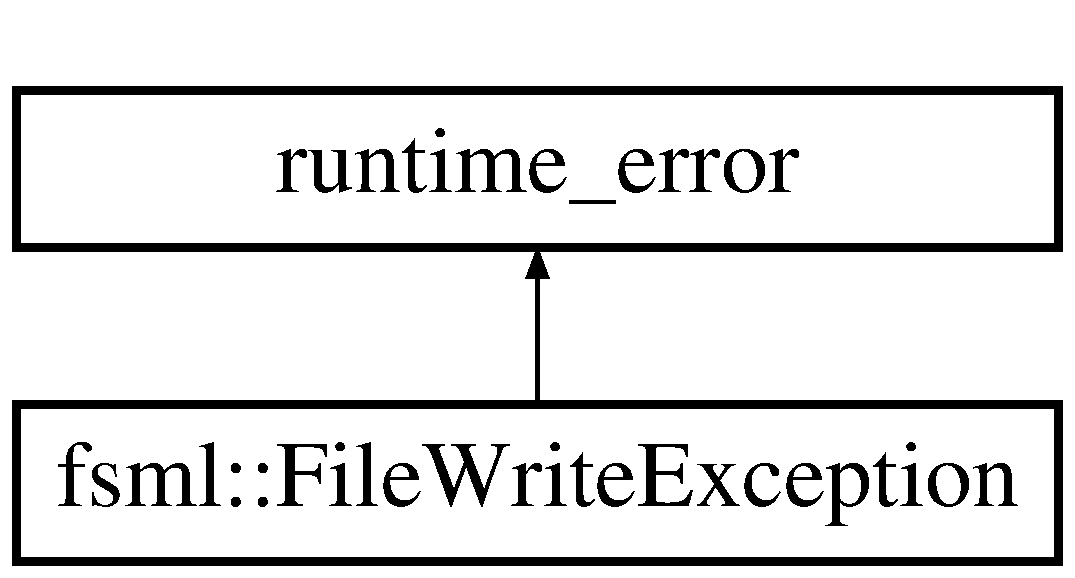
\includegraphics[height=2.000000cm]{structfsml_1_1FileWriteException}
\end{center}
\end{figure}
\subsection*{Public Member Functions}
\begin{DoxyCompactItemize}
\item 
\hypertarget{structfsml_1_1FileWriteException_aa8b9c1d366dbf76392a775279bc2dd19}{{\bfseries File\-Write\-Exception} (const std\-::string \&file)}\label{structfsml_1_1FileWriteException_aa8b9c1d366dbf76392a775279bc2dd19}

\end{DoxyCompactItemize}


\subsection{Detailed Description}
Exception thrown if an error occurs writing to a file. 



The documentation for this struct was generated from the following files\-:\begin{DoxyCompactItemize}
\item 
include/fsml/Exceptions.\-hpp\item 
src/fsml/Exceptions.\-cpp\end{DoxyCompactItemize}

\hypertarget{structfsml_1_1FlatMachine}{\section{fsml\-:\-:Flat\-Machine Struct Reference}
\label{structfsml_1_1FlatMachine}\index{fsml\-::\-Flat\-Machine@{fsml\-::\-Flat\-Machine}}
}


Flat representation of the abstract syntax tree.  




{\ttfamily \#include $<$Flat\-Machine.\-hpp$>$}

\subsection*{Public Member Functions}
\begin{DoxyCompactItemize}
\item 
\hyperlink{structfsml_1_1FlatMachine_a939aa63ea93b644c498cf2e31f67499f}{Flat\-Machine} (const \hyperlink{structfsml_1_1AstMachine}{Ast\-Machine} \&am)
\begin{DoxyCompactList}\small\item\em Constructs a flattened representation of the given abstract syntax tree machine. \end{DoxyCompactList}\item 
\hyperlink{structfsml_1_1FlatMachine_a79e252b2ba388c1064d9570a6df275af}{operator Ast\-Machine} () const 
\begin{DoxyCompactList}\small\item\em Converts this \hyperlink{structfsml_1_1FlatMachine}{Flat\-Machine} into an equivalent, minimal abstract syntax tree. \end{DoxyCompactList}\item 
\hyperlink{structfsml_1_1FlatMachine_a3c50e3140f7629c8c34f2c760522203b}{operator std\-::string} () const 
\begin{DoxyCompactList}\small\item\em Converts this \hyperlink{structfsml_1_1FlatMachine}{Flat\-Machine} into a string. \end{DoxyCompactList}\end{DoxyCompactItemize}
\subsection*{Public Attributes}
\begin{DoxyCompactItemize}
\item 
\hypertarget{structfsml_1_1FlatMachine_a5f3c317f5a3a8f13f10160dcaeef63e3}{std\-::vector$<$ std\-::string $>$ \hyperlink{structfsml_1_1FlatMachine_a5f3c317f5a3a8f13f10160dcaeef63e3}{states}}\label{structfsml_1_1FlatMachine_a5f3c317f5a3a8f13f10160dcaeef63e3}

\begin{DoxyCompactList}\small\item\em The non-\/inital states. \end{DoxyCompactList}\item 
\hypertarget{structfsml_1_1FlatMachine_a3069121ea01eab1cec46590ab186b622}{std\-::vector$<$ std\-::string $>$ \hyperlink{structfsml_1_1FlatMachine_a3069121ea01eab1cec46590ab186b622}{initials}}\label{structfsml_1_1FlatMachine_a3069121ea01eab1cec46590ab186b622}

\begin{DoxyCompactList}\small\item\em The inital states. \end{DoxyCompactList}\item 
\hypertarget{structfsml_1_1FlatMachine_a2fc01c07d6bc3f62fba880e96e538390}{std\-::vector$<$ \hyperlink{structfsml_1_1FlatStep}{Flat\-Step} $>$ \hyperlink{structfsml_1_1FlatMachine_a2fc01c07d6bc3f62fba880e96e538390}{steps}}\label{structfsml_1_1FlatMachine_a2fc01c07d6bc3f62fba880e96e538390}

\begin{DoxyCompactList}\small\item\em The transitions. \end{DoxyCompactList}\end{DoxyCompactItemize}


\subsection{Detailed Description}
Flat representation of the abstract syntax tree. 



\subsection{Constructor \& Destructor Documentation}
\hypertarget{structfsml_1_1FlatMachine_a939aa63ea93b644c498cf2e31f67499f}{\index{fsml\-::\-Flat\-Machine@{fsml\-::\-Flat\-Machine}!Flat\-Machine@{Flat\-Machine}}
\index{Flat\-Machine@{Flat\-Machine}!fsml::FlatMachine@{fsml\-::\-Flat\-Machine}}
\subsubsection[{Flat\-Machine}]{\setlength{\rightskip}{0pt plus 5cm}fsml\-::\-Flat\-Machine\-::\-Flat\-Machine (
\begin{DoxyParamCaption}
\item[{const {\bf Ast\-Machine} \&}]{am}
\end{DoxyParamCaption}
)}}\label{structfsml_1_1FlatMachine_a939aa63ea93b644c498cf2e31f67499f}


Constructs a flattened representation of the given abstract syntax tree machine. 


\begin{DoxyParams}{Parameters}
{\em am} & Abstract syntax tree to generate from. \\
\hline
\end{DoxyParams}


\subsection{Member Function Documentation}
\hypertarget{structfsml_1_1FlatMachine_a79e252b2ba388c1064d9570a6df275af}{\index{fsml\-::\-Flat\-Machine@{fsml\-::\-Flat\-Machine}!operator Ast\-Machine@{operator Ast\-Machine}}
\index{operator Ast\-Machine@{operator Ast\-Machine}!fsml::FlatMachine@{fsml\-::\-Flat\-Machine}}
\subsubsection[{operator Ast\-Machine}]{\setlength{\rightskip}{0pt plus 5cm}fsml\-::\-Flat\-Machine\-::operator {\bf Ast\-Machine} (
\begin{DoxyParamCaption}
{}
\end{DoxyParamCaption}
) const}}\label{structfsml_1_1FlatMachine_a79e252b2ba388c1064d9570a6df275af}


Converts this \hyperlink{structfsml_1_1FlatMachine}{Flat\-Machine} into an equivalent, minimal abstract syntax tree. 

\hypertarget{structfsml_1_1FlatMachine_a3c50e3140f7629c8c34f2c760522203b}{\index{fsml\-::\-Flat\-Machine@{fsml\-::\-Flat\-Machine}!operator std\-::string@{operator std\-::string}}
\index{operator std\-::string@{operator std\-::string}!fsml::FlatMachine@{fsml\-::\-Flat\-Machine}}
\subsubsection[{operator std\-::string}]{\setlength{\rightskip}{0pt plus 5cm}fsml\-::\-Flat\-Machine\-::operator std\-::string (
\begin{DoxyParamCaption}
{}
\end{DoxyParamCaption}
) const}}\label{structfsml_1_1FlatMachine_a3c50e3140f7629c8c34f2c760522203b}


Converts this \hyperlink{structfsml_1_1FlatMachine}{Flat\-Machine} into a string. 



The documentation for this struct was generated from the following files\-:\begin{DoxyCompactItemize}
\item 
include/fsml/Flat\-Machine.\-hpp\item 
src/fsml/Flat\-Machine.\-cpp\end{DoxyCompactItemize}

\hypertarget{structfsml_1_1FlatStep}{\section{fsml\-:\-:Flat\-Step Struct Reference}
\label{structfsml_1_1FlatStep}\index{fsml\-::\-Flat\-Step@{fsml\-::\-Flat\-Step}}
}


Flat representation of a transition.  




{\ttfamily \#include $<$Flat\-Step.\-hpp$>$}

\subsection*{Public Member Functions}
\begin{DoxyCompactItemize}
\item 
\hyperlink{structfsml_1_1FlatStep_a2056fa8fd3e527dd04fffb7011fe3d16}{Flat\-Step} (const std\-::string \&\hyperlink{structfsml_1_1FlatStep_a0d750cd9f657776ffc88627a44d9fdf6}{source}, const std\-::string \&\hyperlink{structfsml_1_1FlatStep_a69f42f7f8091dff898b7944a12cb563e}{input}, const std\-::string \&\hyperlink{structfsml_1_1FlatStep_a910a78d294c31aea42fc23babd361cdb}{action}, const std\-::string \&\hyperlink{structfsml_1_1FlatStep_a2a4242c4ad9b86ce6e1fc638ed4427be}{target})
\begin{DoxyCompactList}\small\item\em Constructs the flattened transition. \end{DoxyCompactList}\item 
\hyperlink{structfsml_1_1FlatStep_aa855ca1535e6dbffb556ee28bd91779f}{operator std\-::string} () const 
\begin{DoxyCompactList}\small\item\em Converts this \hyperlink{structfsml_1_1FlatStep}{Flat\-Step} to a string. \end{DoxyCompactList}\item 
const std\-::string \hyperlink{structfsml_1_1FlatStep_a264b67de20cbd29b079aa46cc332f336}{get\-Step\-Text} () const 
\end{DoxyCompactItemize}
\subsection*{Public Attributes}
\begin{DoxyCompactItemize}
\item 
\hypertarget{structfsml_1_1FlatStep_a0d750cd9f657776ffc88627a44d9fdf6}{std\-::string \hyperlink{structfsml_1_1FlatStep_a0d750cd9f657776ffc88627a44d9fdf6}{source}}\label{structfsml_1_1FlatStep_a0d750cd9f657776ffc88627a44d9fdf6}

\begin{DoxyCompactList}\small\item\em The source state. \end{DoxyCompactList}\item 
\hypertarget{structfsml_1_1FlatStep_a69f42f7f8091dff898b7944a12cb563e}{std\-::string \hyperlink{structfsml_1_1FlatStep_a69f42f7f8091dff898b7944a12cb563e}{input}}\label{structfsml_1_1FlatStep_a69f42f7f8091dff898b7944a12cb563e}

\begin{DoxyCompactList}\small\item\em The input name. \end{DoxyCompactList}\item 
\hypertarget{structfsml_1_1FlatStep_a910a78d294c31aea42fc23babd361cdb}{std\-::string \hyperlink{structfsml_1_1FlatStep_a910a78d294c31aea42fc23babd361cdb}{action}}\label{structfsml_1_1FlatStep_a910a78d294c31aea42fc23babd361cdb}

\begin{DoxyCompactList}\small\item\em The action name or empty string for no action. \end{DoxyCompactList}\item 
\hypertarget{structfsml_1_1FlatStep_a2a4242c4ad9b86ce6e1fc638ed4427be}{std\-::string \hyperlink{structfsml_1_1FlatStep_a2a4242c4ad9b86ce6e1fc638ed4427be}{target}}\label{structfsml_1_1FlatStep_a2a4242c4ad9b86ce6e1fc638ed4427be}

\begin{DoxyCompactList}\small\item\em The target state. \end{DoxyCompactList}\end{DoxyCompactItemize}


\subsection{Detailed Description}
Flat representation of a transition. 



\subsection{Constructor \& Destructor Documentation}
\hypertarget{structfsml_1_1FlatStep_a2056fa8fd3e527dd04fffb7011fe3d16}{\index{fsml\-::\-Flat\-Step@{fsml\-::\-Flat\-Step}!Flat\-Step@{Flat\-Step}}
\index{Flat\-Step@{Flat\-Step}!fsml::FlatStep@{fsml\-::\-Flat\-Step}}
\subsubsection[{Flat\-Step}]{\setlength{\rightskip}{0pt plus 5cm}fsml\-::\-Flat\-Step\-::\-Flat\-Step (
\begin{DoxyParamCaption}
\item[{const std\-::string \&}]{source, }
\item[{const std\-::string \&}]{input, }
\item[{const std\-::string \&}]{action, }
\item[{const std\-::string \&}]{target}
\end{DoxyParamCaption}
)}}\label{structfsml_1_1FlatStep_a2056fa8fd3e527dd04fffb7011fe3d16}


Constructs the flattened transition. 


\begin{DoxyParams}{Parameters}
{\em source} & Source state. \\
\hline
{\em input} & Input name. \\
\hline
{\em action} & \hyperlink{classfsml_1_1Action}{Action} name or empty string for no action. \\
\hline
{\em target} & Target state or empty string for source being target. \\
\hline
\end{DoxyParams}


\subsection{Member Function Documentation}
\hypertarget{structfsml_1_1FlatStep_a264b67de20cbd29b079aa46cc332f336}{\index{fsml\-::\-Flat\-Step@{fsml\-::\-Flat\-Step}!get\-Step\-Text@{get\-Step\-Text}}
\index{get\-Step\-Text@{get\-Step\-Text}!fsml::FlatStep@{fsml\-::\-Flat\-Step}}
\subsubsection[{get\-Step\-Text}]{\setlength{\rightskip}{0pt plus 5cm}const string fsml\-::\-Flat\-Step\-::get\-Step\-Text (
\begin{DoxyParamCaption}
{}
\end{DoxyParamCaption}
) const}}\label{structfsml_1_1FlatStep_a264b67de20cbd29b079aa46cc332f336}
\begin{DoxyReturn}{Returns}
The text for the transition (input or input/action). 
\end{DoxyReturn}
\hypertarget{structfsml_1_1FlatStep_aa855ca1535e6dbffb556ee28bd91779f}{\index{fsml\-::\-Flat\-Step@{fsml\-::\-Flat\-Step}!operator std\-::string@{operator std\-::string}}
\index{operator std\-::string@{operator std\-::string}!fsml::FlatStep@{fsml\-::\-Flat\-Step}}
\subsubsection[{operator std\-::string}]{\setlength{\rightskip}{0pt plus 5cm}fsml\-::\-Flat\-Step\-::operator std\-::string (
\begin{DoxyParamCaption}
{}
\end{DoxyParamCaption}
) const}}\label{structfsml_1_1FlatStep_aa855ca1535e6dbffb556ee28bd91779f}


Converts this \hyperlink{structfsml_1_1FlatStep}{Flat\-Step} to a string. 



The documentation for this struct was generated from the following files\-:\begin{DoxyCompactItemize}
\item 
include/fsml/Flat\-Step.\-hpp\item 
src/fsml/Flat\-Step.\-cpp\end{DoxyCompactItemize}

\hypertarget{structfsml_1_1InitialStateException}{\section{fsml\-:\-:Initial\-State\-Exception Struct Reference}
\label{structfsml_1_1InitialStateException}\index{fsml\-::\-Initial\-State\-Exception@{fsml\-::\-Initial\-State\-Exception}}
}
Inheritance diagram for fsml\-:\-:Initial\-State\-Exception\-:\begin{figure}[H]
\begin{center}
\leavevmode
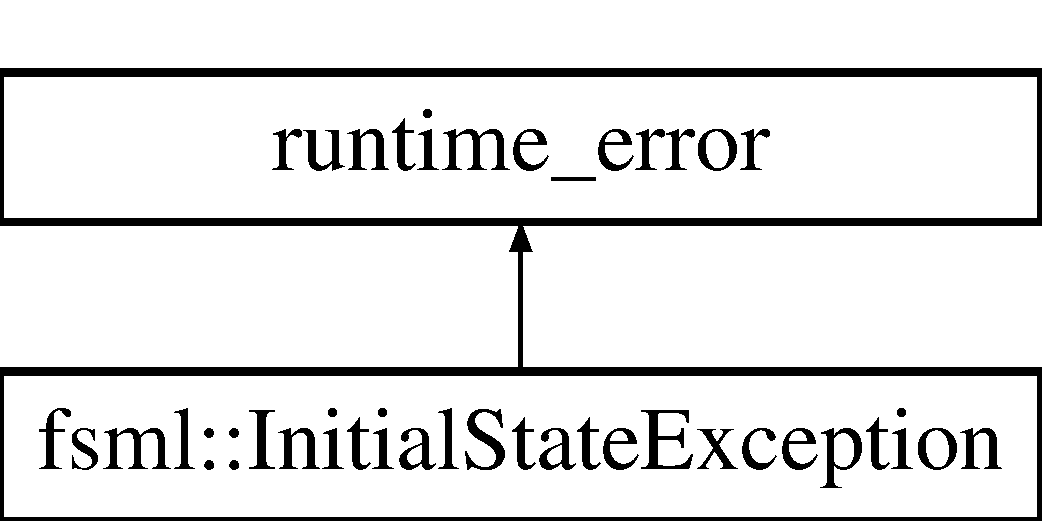
\includegraphics[height=2.000000cm]{structfsml_1_1InitialStateException}
\end{center}
\end{figure}
\subsection*{Public Member Functions}
\begin{DoxyCompactItemize}
\item 
\hypertarget{structfsml_1_1InitialStateException_ae4cf2e419f5f5d221af4d7de2907dbb5}{{\bfseries Initial\-State\-Exception} (const std\-::vector$<$ std\-::string $>$ \&states)}\label{structfsml_1_1InitialStateException_ae4cf2e419f5f5d221af4d7de2907dbb5}

\end{DoxyCompactItemize}


The documentation for this struct was generated from the following files\-:\begin{DoxyCompactItemize}
\item 
include/fsml/Exceptions.\-hpp\item 
src/fsml/Exceptions.\-cpp\end{DoxyCompactItemize}

\hypertarget{structfsml_1_1InvalidInputException}{\section{fsml\-:\-:Invalid\-Input\-Exception Struct Reference}
\label{structfsml_1_1InvalidInputException}\index{fsml\-::\-Invalid\-Input\-Exception@{fsml\-::\-Invalid\-Input\-Exception}}
}
Inheritance diagram for fsml\-:\-:Invalid\-Input\-Exception\-:\begin{figure}[H]
\begin{center}
\leavevmode
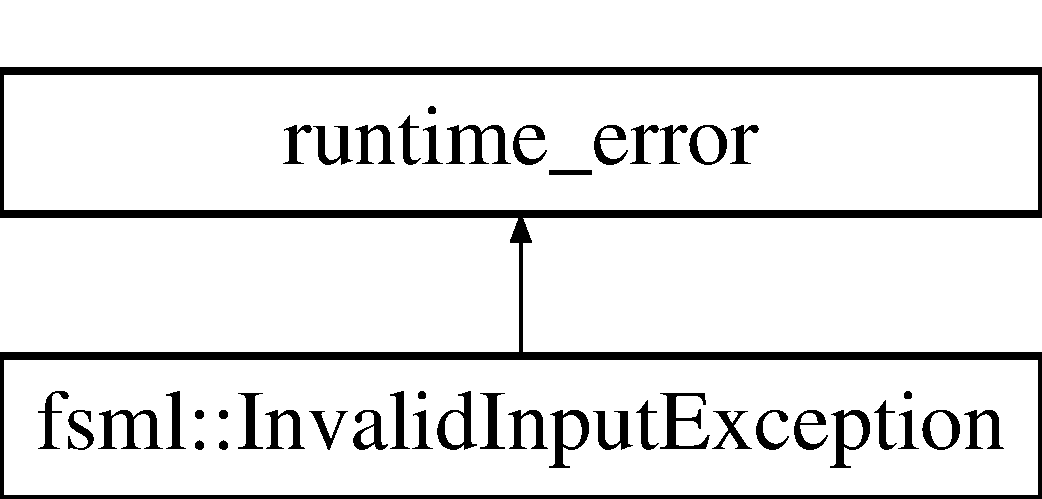
\includegraphics[height=2.000000cm]{structfsml_1_1InvalidInputException}
\end{center}
\end{figure}
\subsection*{Public Member Functions}
\begin{DoxyCompactItemize}
\item 
\hypertarget{structfsml_1_1InvalidInputException_aa7373c1db918bf47817d2d85e089ee50}{{\bfseries Invalid\-Input\-Exception} (const std\-::string \&state, const std\-::string \&input)}\label{structfsml_1_1InvalidInputException_aa7373c1db918bf47817d2d85e089ee50}

\end{DoxyCompactItemize}


The documentation for this struct was generated from the following files\-:\begin{DoxyCompactItemize}
\item 
include/fsml/Exceptions.\-hpp\item 
src/fsml/Exceptions.\-cpp\end{DoxyCompactItemize}

\hypertarget{classfsml_1_1Machine}{\section{fsml\-:\-:Machine Class Reference}
\label{classfsml_1_1Machine}\index{fsml\-::\-Machine@{fsml\-::\-Machine}}
}


Represents a simulatable final state machine.  




{\ttfamily \#include $<$Machine.\-hpp$>$}

\subsection*{Public Member Functions}
\begin{DoxyCompactItemize}
\item 
\hyperlink{classfsml_1_1Machine_a0666d3b6834e968bd0fe1461164de7ef}{Machine} (const \hyperlink{structfsml_1_1FlatMachine}{Flat\-Machine} \&fm)
\begin{DoxyCompactList}\small\item\em Constructs and validates a \hyperlink{classfsml_1_1Machine}{Machine} from the given \hyperlink{structfsml_1_1FlatMachine}{Flat\-Machine}. \end{DoxyCompactList}\item 
\hyperlink{classfsml_1_1Machine_a0c60fab103e0e65343c729ed3502ebac}{Machine} (const std\-::vector$<$ std\-::string $>$ \&initials, const std\-::vector$<$ std\-::string $>$ \&states, const std\-::vector$<$ \hyperlink{structfsml_1_1FlatStep}{Flat\-Step} $>$ \&steps)
\begin{DoxyCompactList}\small\item\em Constructs and validates a \hyperlink{classfsml_1_1Machine}{Machine} from the given parameters. \end{DoxyCompactList}\item 
virtual \hyperlink{classfsml_1_1Machine}{Machine} \& \hyperlink{classfsml_1_1Machine_a4c02303acf2c3bd89ffc6ceda604b02d}{operator$<$$<$} (const std\-::string \&input)
\begin{DoxyCompactList}\small\item\em Feeds the given input into the \hyperlink{classfsml_1_1Machine}{Machine}. \end{DoxyCompactList}\item 
\hypertarget{classfsml_1_1Machine_a146384b88619887f03613f439781e9e0}{virtual {\bfseries operator Flat\-Machine} () const }\label{classfsml_1_1Machine_a146384b88619887f03613f439781e9e0}

\item 
virtual const \\*
std\-::unordered\-\_\-set$<$ const \\*
\hyperlink{classfsml_1_1State}{State} $\ast$ $>$ \hyperlink{classfsml_1_1Machine_a7d184c839fe996141a692152b9b37e0a}{reachable\-From} (const \hyperlink{classfsml_1_1State}{State} $\ast$const start) const 
\begin{DoxyCompactList}\small\item\em Gathers the States reachable from the given \hyperlink{classfsml_1_1State}{State}. \end{DoxyCompactList}\item 
virtual void \hyperlink{classfsml_1_1Machine_a51b789ab95db22995529818bed9fef20}{register\-At} (const std\-::string \&action, const Action\-Function \&func)
\begin{DoxyCompactList}\small\item\em Registers the given function with the given action. \end{DoxyCompactList}\item 
virtual const \hyperlink{classfsml_1_1State}{State} \& \hyperlink{classfsml_1_1Machine_a5bce113183b6d59b652b33f4369bb45c}{get\-Current\-State} () const 
\end{DoxyCompactItemize}
\subsection*{Protected Member Functions}
\begin{DoxyCompactItemize}
\item 
void \hyperlink{classfsml_1_1Machine_a863ac1a16a82e0fc0a8e85553061686f}{add\-Step} (const std\-::string \&source\-Id, const std\-::string \&input, const std\-::string \&action\-Id, const std\-::string \&target\-Id)
\begin{DoxyCompactList}\small\item\em Constructs a step from the given parameters and adds it to the source state. \end{DoxyCompactList}\end{DoxyCompactItemize}
\subsection*{Protected Attributes}
\begin{DoxyCompactItemize}
\item 
\hypertarget{classfsml_1_1Machine_a02a00a80f4f77625cd1fbcb2314d3c21}{std\-::unordered\-\_\-map\\*
$<$ std\-::string, \hyperlink{classfsml_1_1Action}{Action} $>$ \hyperlink{classfsml_1_1Machine_a02a00a80f4f77625cd1fbcb2314d3c21}{action\-Map}}\label{classfsml_1_1Machine_a02a00a80f4f77625cd1fbcb2314d3c21}

\begin{DoxyCompactList}\small\item\em Maps actions to their respective name. \end{DoxyCompactList}\item 
\hypertarget{classfsml_1_1Machine_a8d777492e8e8b0e79b041444f386c319}{std\-::unordered\-\_\-map\\*
$<$ std\-::string, \hyperlink{classfsml_1_1State}{State} $>$ \hyperlink{classfsml_1_1Machine_a8d777492e8e8b0e79b041444f386c319}{state\-Map}}\label{classfsml_1_1Machine_a8d777492e8e8b0e79b041444f386c319}

\begin{DoxyCompactList}\small\item\em Maps states to their respective name. \end{DoxyCompactList}\item 
\hypertarget{classfsml_1_1Machine_a8c4e7bc3c75c8b40a28d0b33a457be9d}{\hyperlink{classfsml_1_1State}{State} $\ast$ \hyperlink{classfsml_1_1Machine_a8c4e7bc3c75c8b40a28d0b33a457be9d}{current}}\label{classfsml_1_1Machine_a8c4e7bc3c75c8b40a28d0b33a457be9d}

\begin{DoxyCompactList}\small\item\em The current \hyperlink{classfsml_1_1State}{State}. \end{DoxyCompactList}\end{DoxyCompactItemize}


\subsection{Detailed Description}
Represents a simulatable final state machine. 



\subsection{Constructor \& Destructor Documentation}
\hypertarget{classfsml_1_1Machine_a0666d3b6834e968bd0fe1461164de7ef}{\index{fsml\-::\-Machine@{fsml\-::\-Machine}!Machine@{Machine}}
\index{Machine@{Machine}!fsml::Machine@{fsml\-::\-Machine}}
\subsubsection[{Machine}]{\setlength{\rightskip}{0pt plus 5cm}fsml\-::\-Machine\-::\-Machine (
\begin{DoxyParamCaption}
\item[{const {\bf Flat\-Machine} \&}]{fm}
\end{DoxyParamCaption}
)}}\label{classfsml_1_1Machine_a0666d3b6834e968bd0fe1461164de7ef}


Constructs and validates a \hyperlink{classfsml_1_1Machine}{Machine} from the given \hyperlink{structfsml_1_1FlatMachine}{Flat\-Machine}. 


\begin{DoxyParams}{Parameters}
{\em fm} & The \hyperlink{structfsml_1_1FlatMachine}{Flat\-Machine}. \\
\hline
\end{DoxyParams}
\begin{DoxyReturn}{Returns}
A \hyperlink{classfsml_1_1Machine}{Machine} corresponding to the given \hyperlink{structfsml_1_1FlatMachine}{Flat\-Machine}, if it is valid. 
\end{DoxyReturn}

\begin{DoxyExceptions}{Exceptions}
{\em \hyperlink{structfsml_1_1InitialStateException}{Initial\-State\-Exception}} & if no or more then one inital state is given. \\
\hline
{\em \hyperlink{structfsml_1_1UniqueException}{Unique\-Exception}} & if a state is defined more than once. \\
\hline
{\em \hyperlink{structfsml_1_1ReachableException}{Reachable\-Exception}} & if a state is not reachable from intial state. \\
\hline
{\em \hyperlink{structfsml_1_1ResolvableException}{Resolvable\-Exception}} & if target state in a transition does not exist. \\
\hline
{\em \hyperlink{structfsml_1_1DeterministicException}{Deterministic\-Exception}} & if an input in a state is not distinct. \\
\hline
\end{DoxyExceptions}
\hypertarget{classfsml_1_1Machine_a0c60fab103e0e65343c729ed3502ebac}{\index{fsml\-::\-Machine@{fsml\-::\-Machine}!Machine@{Machine}}
\index{Machine@{Machine}!fsml::Machine@{fsml\-::\-Machine}}
\subsubsection[{Machine}]{\setlength{\rightskip}{0pt plus 5cm}fsml\-::\-Machine\-::\-Machine (
\begin{DoxyParamCaption}
\item[{const std\-::vector$<$ std\-::string $>$ \&}]{initials, }
\item[{const std\-::vector$<$ std\-::string $>$ \&}]{states, }
\item[{const std\-::vector$<$ {\bf Flat\-Step} $>$ \&}]{steps}
\end{DoxyParamCaption}
)}}\label{classfsml_1_1Machine_a0c60fab103e0e65343c729ed3502ebac}


Constructs and validates a \hyperlink{classfsml_1_1Machine}{Machine} from the given parameters. 


\begin{DoxyParams}{Parameters}
{\em initials} & The initial states. \\
\hline
{\em states} & The non-\/inital states. \\
\hline
{\em steps} & The transitions. \\
\hline
\end{DoxyParams}
\begin{DoxyReturn}{Returns}
A \hyperlink{classfsml_1_1Machine}{Machine} corresponding to the given parameters, if they are valid. 
\end{DoxyReturn}

\begin{DoxyExceptions}{Exceptions}
{\em \hyperlink{structfsml_1_1InitialStateException}{Initial\-State\-Exception}} & if no or more then one inital state is given. \\
\hline
{\em \hyperlink{structfsml_1_1UniqueException}{Unique\-Exception}} & if a state is defined more than once. \\
\hline
{\em \hyperlink{structfsml_1_1ReachableException}{Reachable\-Exception}} & if a state is not reachable from intial state. \\
\hline
{\em \hyperlink{structfsml_1_1ResolvableException}{Resolvable\-Exception}} & if target state in a transition does not exist. \\
\hline
{\em \hyperlink{structfsml_1_1DeterministicException}{Deterministic\-Exception}} & if an input in a state is not distinct. \\
\hline
\end{DoxyExceptions}


\subsection{Member Function Documentation}
\hypertarget{classfsml_1_1Machine_a863ac1a16a82e0fc0a8e85553061686f}{\index{fsml\-::\-Machine@{fsml\-::\-Machine}!add\-Step@{add\-Step}}
\index{add\-Step@{add\-Step}!fsml::Machine@{fsml\-::\-Machine}}
\subsubsection[{add\-Step}]{\setlength{\rightskip}{0pt plus 5cm}void fsml\-::\-Machine\-::add\-Step (
\begin{DoxyParamCaption}
\item[{const std\-::string \&}]{source\-Id, }
\item[{const std\-::string \&}]{input, }
\item[{const std\-::string \&}]{action\-Id, }
\item[{const std\-::string \&}]{target\-Id}
\end{DoxyParamCaption}
)\hspace{0.3cm}{\ttfamily [protected]}}}\label{classfsml_1_1Machine_a863ac1a16a82e0fc0a8e85553061686f}


Constructs a step from the given parameters and adds it to the source state. 


\begin{DoxyParams}{Parameters}
{\em sourc\-Id} & The source state's name. \\
\hline
{\em input} & The input name. \\
\hline
{\em action\-Id} & The action name. \\
\hline
{\em target\-Id} & The target state's name. \\
\hline
\end{DoxyParams}

\begin{DoxyExceptions}{Exceptions}
{\em \hyperlink{structfsml_1_1ResolvableException}{Resolvable\-Exception}} & if target does not exist. \\
\hline
{\em \hyperlink{structfsml_1_1DeterministicException}{Deterministic\-Exception}} & if there is more than one possible transition for the given input. \\
\hline
\end{DoxyExceptions}
\hypertarget{classfsml_1_1Machine_a5bce113183b6d59b652b33f4369bb45c}{\index{fsml\-::\-Machine@{fsml\-::\-Machine}!get\-Current\-State@{get\-Current\-State}}
\index{get\-Current\-State@{get\-Current\-State}!fsml::Machine@{fsml\-::\-Machine}}
\subsubsection[{get\-Current\-State}]{\setlength{\rightskip}{0pt plus 5cm}const {\bf State} \& fsml\-::\-Machine\-::get\-Current\-State (
\begin{DoxyParamCaption}
{}
\end{DoxyParamCaption}
) const\hspace{0.3cm}{\ttfamily [virtual]}}}\label{classfsml_1_1Machine_a5bce113183b6d59b652b33f4369bb45c}
\begin{DoxyReturn}{Returns}
The current \hyperlink{classfsml_1_1State}{State}. 
\end{DoxyReturn}
\hypertarget{classfsml_1_1Machine_a4c02303acf2c3bd89ffc6ceda604b02d}{\index{fsml\-::\-Machine@{fsml\-::\-Machine}!operator$<$$<$@{operator$<$$<$}}
\index{operator$<$$<$@{operator$<$$<$}!fsml::Machine@{fsml\-::\-Machine}}
\subsubsection[{operator$<$$<$}]{\setlength{\rightskip}{0pt plus 5cm}{\bf Machine} \& fsml\-::\-Machine\-::operator$<$$<$ (
\begin{DoxyParamCaption}
\item[{const std\-::string \&}]{input}
\end{DoxyParamCaption}
)\hspace{0.3cm}{\ttfamily [virtual]}}}\label{classfsml_1_1Machine_a4c02303acf2c3bd89ffc6ceda604b02d}


Feeds the given input into the \hyperlink{classfsml_1_1Machine}{Machine}. 

The current \hyperlink{classfsml_1_1State}{State} will attempt to execute the corresponding transition and change the current \hyperlink{classfsml_1_1State}{State}. If an action is triggered, the registered function will be called, if it exists. 
\begin{DoxyParams}{Parameters}
{\em input} & The input name. \\
\hline
\end{DoxyParams}
\begin{DoxyReturn}{Returns}
The \hyperlink{classfsml_1_1Machine}{Machine} itself so that input can be chained. 
\end{DoxyReturn}

\begin{DoxyExceptions}{Exceptions}
{\em \hyperlink{structfsml_1_1InvalidInputException}{Invalid\-Input\-Exception}} & if the current \hyperlink{classfsml_1_1State}{State} cannot handle the input. The current \hyperlink{classfsml_1_1State}{State} will not be changed. \\
\hline
\end{DoxyExceptions}
\hypertarget{classfsml_1_1Machine_a7d184c839fe996141a692152b9b37e0a}{\index{fsml\-::\-Machine@{fsml\-::\-Machine}!reachable\-From@{reachable\-From}}
\index{reachable\-From@{reachable\-From}!fsml::Machine@{fsml\-::\-Machine}}
\subsubsection[{reachable\-From}]{\setlength{\rightskip}{0pt plus 5cm}const unordered\-\_\-set$<$ const {\bf State} $\ast$ $>$ fsml\-::\-Machine\-::reachable\-From (
\begin{DoxyParamCaption}
\item[{const {\bf State} $\ast$const}]{start}
\end{DoxyParamCaption}
) const\hspace{0.3cm}{\ttfamily [virtual]}}}\label{classfsml_1_1Machine_a7d184c839fe996141a692152b9b37e0a}


Gathers the States reachable from the given \hyperlink{classfsml_1_1State}{State}. 


\begin{DoxyParams}{Parameters}
{\em start} & The \hyperlink{classfsml_1_1State}{State} from which to start from. \\
\hline
\end{DoxyParams}
\begin{DoxyReturn}{Returns}
An unordered set of states reachable from start. 
\end{DoxyReturn}
\hypertarget{classfsml_1_1Machine_a51b789ab95db22995529818bed9fef20}{\index{fsml\-::\-Machine@{fsml\-::\-Machine}!register\-At@{register\-At}}
\index{register\-At@{register\-At}!fsml::Machine@{fsml\-::\-Machine}}
\subsubsection[{register\-At}]{\setlength{\rightskip}{0pt plus 5cm}void fsml\-::\-Machine\-::register\-At (
\begin{DoxyParamCaption}
\item[{const std\-::string \&}]{action, }
\item[{const Action\-Function \&}]{func}
\end{DoxyParamCaption}
)\hspace{0.3cm}{\ttfamily [virtual]}}}\label{classfsml_1_1Machine_a51b789ab95db22995529818bed9fef20}


Registers the given function with the given action. 


\begin{DoxyParams}{Parameters}
{\em action} & The action name. \\
\hline
{\em func} & The function to register. \\
\hline
\end{DoxyParams}

\begin{DoxyExceptions}{Exceptions}
{\em out\-\_\-of\-\_\-range} & if the action does not exist. \\
\hline
\end{DoxyExceptions}


The documentation for this class was generated from the following files\-:\begin{DoxyCompactItemize}
\item 
include/fsml/Machine.\-hpp\item 
src/fsml/Machine.\-cpp\end{DoxyCompactItemize}

\hypertarget{structfsml_1_1ParserException}{\section{fsml\-:\-:Parser\-Exception Struct Reference}
\label{structfsml_1_1ParserException}\index{fsml\-::\-Parser\-Exception@{fsml\-::\-Parser\-Exception}}
}


Exception thrown if parsing fails.  




{\ttfamily \#include $<$Exceptions.\-hpp$>$}

Inheritance diagram for fsml\-:\-:Parser\-Exception\-:\begin{figure}[H]
\begin{center}
\leavevmode
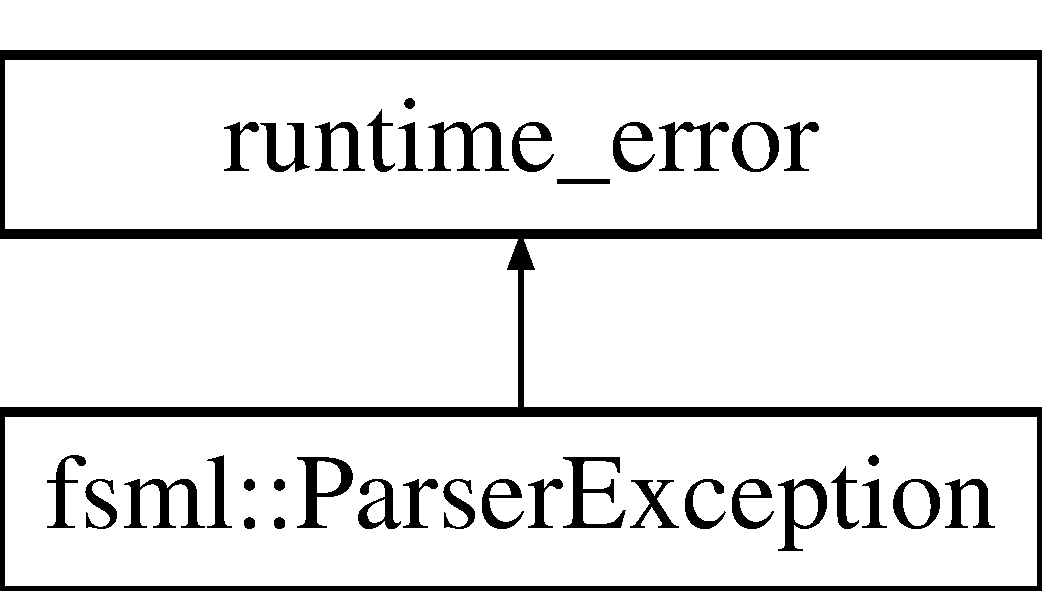
\includegraphics[height=2.000000cm]{structfsml_1_1ParserException}
\end{center}
\end{figure}
\subsection*{Public Member Functions}
\begin{DoxyCompactItemize}
\item 
\hypertarget{structfsml_1_1ParserException_a022b04432a881271696b5e9e7f9df5af}{{\bfseries Parser\-Exception} (const std\-::string \&file)}\label{structfsml_1_1ParserException_a022b04432a881271696b5e9e7f9df5af}

\end{DoxyCompactItemize}


\subsection{Detailed Description}
Exception thrown if parsing fails. 



The documentation for this struct was generated from the following files\-:\begin{DoxyCompactItemize}
\item 
include/fsml/Exceptions.\-hpp\item 
src/fsml/Exceptions.\-cpp\end{DoxyCompactItemize}

\hypertarget{structfsml_1_1ReachableException}{\section{fsml\-:\-:Reachable\-Exception Struct Reference}
\label{structfsml_1_1ReachableException}\index{fsml\-::\-Reachable\-Exception@{fsml\-::\-Reachable\-Exception}}
}


Exception thrown if not all States in a \hyperlink{classfsml_1_1Machine}{Machine} are reachable.  




{\ttfamily \#include $<$Exceptions.\-hpp$>$}

Inheritance diagram for fsml\-:\-:Reachable\-Exception\-:\begin{figure}[H]
\begin{center}
\leavevmode
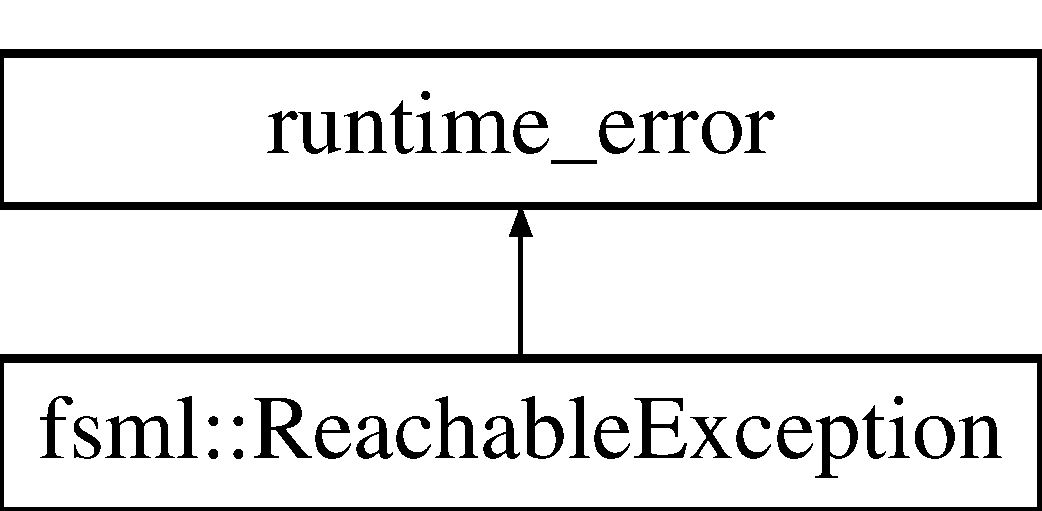
\includegraphics[height=2.000000cm]{structfsml_1_1ReachableException}
\end{center}
\end{figure}
\subsection*{Public Member Functions}
\begin{DoxyCompactItemize}
\item 
\hypertarget{structfsml_1_1ReachableException_a10ee53b62caeefb43be52d96420d0798}{{\bfseries Reachable\-Exception} (const std\-::pair$<$ std\-::vector$<$ std\-::string $>$, std\-::vector$<$ std\-::string $>$$>$ \&states)}\label{structfsml_1_1ReachableException_a10ee53b62caeefb43be52d96420d0798}

\end{DoxyCompactItemize}
\subsection*{Public Attributes}
\begin{DoxyCompactItemize}
\item 
\hypertarget{structfsml_1_1ReachableException_a6101b6deeeaba35c21944812ab71bf5d}{std\-::vector$<$ std\-::string $>$ {\bfseries reachable}}\label{structfsml_1_1ReachableException_a6101b6deeeaba35c21944812ab71bf5d}

\end{DoxyCompactItemize}


\subsection{Detailed Description}
Exception thrown if not all States in a \hyperlink{classfsml_1_1Machine}{Machine} are reachable. 



The documentation for this struct was generated from the following files\-:\begin{DoxyCompactItemize}
\item 
include/fsml/Exceptions.\-hpp\item 
src/fsml/Exceptions.\-cpp\end{DoxyCompactItemize}

\hypertarget{structfsml_1_1ResolvableException}{\section{fsml\-:\-:Resolvable\-Exception Struct Reference}
\label{structfsml_1_1ResolvableException}\index{fsml\-::\-Resolvable\-Exception@{fsml\-::\-Resolvable\-Exception}}
}


Exception thrown if the target of a \hyperlink{classfsml_1_1Step}{Step} is not resolvable.  




{\ttfamily \#include $<$Exceptions.\-hpp$>$}

Inheritance diagram for fsml\-:\-:Resolvable\-Exception\-:\begin{figure}[H]
\begin{center}
\leavevmode
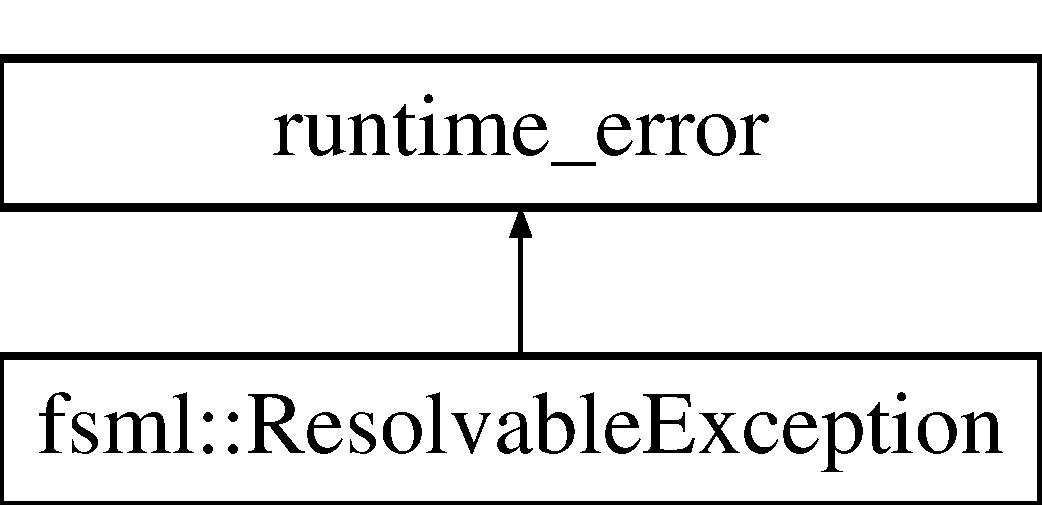
\includegraphics[height=2.000000cm]{structfsml_1_1ResolvableException}
\end{center}
\end{figure}
\subsection*{Public Member Functions}
\begin{DoxyCompactItemize}
\item 
\hypertarget{structfsml_1_1ResolvableException_abe17276c3a06e7a331d9e3db7d480af8}{{\bfseries Resolvable\-Exception} (const std\-::string \&target, const std\-::string \&state)}\label{structfsml_1_1ResolvableException_abe17276c3a06e7a331d9e3db7d480af8}

\end{DoxyCompactItemize}


\subsection{Detailed Description}
Exception thrown if the target of a \hyperlink{classfsml_1_1Step}{Step} is not resolvable. 



The documentation for this struct was generated from the following files\-:\begin{DoxyCompactItemize}
\item 
include/fsml/Exceptions.\-hpp\item 
src/fsml/Exceptions.\-cpp\end{DoxyCompactItemize}

\hypertarget{classfsml_1_1State}{\section{fsml\-:\-:State Class Reference}
\label{classfsml_1_1State}\index{fsml\-::\-State@{fsml\-::\-State}}
}


Represents a \hyperlink{classfsml_1_1Machine}{Machine}'s state.  




{\ttfamily \#include $<$State.\-hpp$>$}

\subsection*{Public Member Functions}
\begin{DoxyCompactItemize}
\item 
\hyperlink{classfsml_1_1State_a22711ba81bad4eb0b4a98b17a45cfd36}{State} (const std\-::string \&\hyperlink{classfsml_1_1State_a4acc37de347d0e4a66d6470a4d6ebcf7}{id}, const bool \&\hyperlink{classfsml_1_1State_aeb0c3fe997b186b77e3c363709a1bfea}{initial}=false)
\begin{DoxyCompactList}\small\item\em Constructs a new \hyperlink{classfsml_1_1State}{State} with the given id. \end{DoxyCompactList}\item 
virtual bool \hyperlink{classfsml_1_1State_a0a28f6f4a995313d9bc85d1fdf51fb9b}{add\-Step} (const std\-::string \&input, const \hyperlink{classfsml_1_1Step}{Step} \&\hyperlink{classfsml_1_1State_a0c7aafd6216a785c159e70f00a12d3f8}{step})
\begin{DoxyCompactList}\small\item\em Attemps to add the given transition to this \hyperlink{classfsml_1_1State}{State}. \end{DoxyCompactList}\item 
virtual \hyperlink{classfsml_1_1State}{State} $\ast$ \hyperlink{classfsml_1_1State_a0c7aafd6216a785c159e70f00a12d3f8}{step} (const std\-::string \&input)
\begin{DoxyCompactList}\small\item\em Attempts to execute the transition corresponding to the given input. \end{DoxyCompactList}\item 
virtual const bool \& \hyperlink{classfsml_1_1State_a2cbbbb658b8d6da4b6b0f0a4e97fed7b}{is\-Initial} () const 
\item 
virtual const std\-::string \& \hyperlink{classfsml_1_1State_af13128f0b9cdf6433f4307bb16159477}{get\-Id} () const 
\item 
virtual const \\*
std\-::unordered\-\_\-map\\*
$<$ std\-::string, \hyperlink{classfsml_1_1Step}{Step} $>$ \& \hyperlink{classfsml_1_1State_ad96fe3074f0c3d8bd3dcb9a7cd7e25ed}{get\-Steps} () const 
\end{DoxyCompactItemize}
\subsection*{Protected Attributes}
\begin{DoxyCompactItemize}
\item 
\hypertarget{classfsml_1_1State_aeb0c3fe997b186b77e3c363709a1bfea}{const bool \hyperlink{classfsml_1_1State_aeb0c3fe997b186b77e3c363709a1bfea}{initial}}\label{classfsml_1_1State_aeb0c3fe997b186b77e3c363709a1bfea}

\begin{DoxyCompactList}\small\item\em The \hyperlink{classfsml_1_1State}{State}'s initialness. \end{DoxyCompactList}\item 
\hypertarget{classfsml_1_1State_a4acc37de347d0e4a66d6470a4d6ebcf7}{const std\-::string \hyperlink{classfsml_1_1State_a4acc37de347d0e4a66d6470a4d6ebcf7}{id}}\label{classfsml_1_1State_a4acc37de347d0e4a66d6470a4d6ebcf7}

\begin{DoxyCompactList}\small\item\em The \hyperlink{classfsml_1_1State}{State}'s id. \end{DoxyCompactList}\item 
\hypertarget{classfsml_1_1State_af9c12ff54dd9712d43b3a10609445642}{std\-::unordered\-\_\-map\\*
$<$ std\-::string, \hyperlink{classfsml_1_1Step}{Step} $>$ \hyperlink{classfsml_1_1State_af9c12ff54dd9712d43b3a10609445642}{steps}}\label{classfsml_1_1State_af9c12ff54dd9712d43b3a10609445642}

\begin{DoxyCompactList}\small\item\em The \hyperlink{classfsml_1_1State}{State}'s transitions. \end{DoxyCompactList}\end{DoxyCompactItemize}


\subsection{Detailed Description}
Represents a \hyperlink{classfsml_1_1Machine}{Machine}'s state. 



\subsection{Constructor \& Destructor Documentation}
\hypertarget{classfsml_1_1State_a22711ba81bad4eb0b4a98b17a45cfd36}{\index{fsml\-::\-State@{fsml\-::\-State}!State@{State}}
\index{State@{State}!fsml::State@{fsml\-::\-State}}
\subsubsection[{State}]{\setlength{\rightskip}{0pt plus 5cm}fsml\-::\-State\-::\-State (
\begin{DoxyParamCaption}
\item[{const std\-::string \&}]{id, }
\item[{const bool \&}]{initial = {\ttfamily false}}
\end{DoxyParamCaption}
)}}\label{classfsml_1_1State_a22711ba81bad4eb0b4a98b17a45cfd36}


Constructs a new \hyperlink{classfsml_1_1State}{State} with the given id. 


\begin{DoxyParams}{Parameters}
{\em id} & The \hyperlink{classfsml_1_1State}{State}'s name. \\
\hline
\end{DoxyParams}


\subsection{Member Function Documentation}
\hypertarget{classfsml_1_1State_a0a28f6f4a995313d9bc85d1fdf51fb9b}{\index{fsml\-::\-State@{fsml\-::\-State}!add\-Step@{add\-Step}}
\index{add\-Step@{add\-Step}!fsml::State@{fsml\-::\-State}}
\subsubsection[{add\-Step}]{\setlength{\rightskip}{0pt plus 5cm}bool fsml\-::\-State\-::add\-Step (
\begin{DoxyParamCaption}
\item[{const std\-::string \&}]{input, }
\item[{const {\bf Step} \&}]{step}
\end{DoxyParamCaption}
)\hspace{0.3cm}{\ttfamily [virtual]}}}\label{classfsml_1_1State_a0a28f6f4a995313d9bc85d1fdf51fb9b}


Attemps to add the given transition to this \hyperlink{classfsml_1_1State}{State}. 


\begin{DoxyParams}{Parameters}
{\em input} & The input name. \\
\hline
{\em step} & The transition. \\
\hline
\end{DoxyParams}
\begin{DoxyReturn}{Returns}
false, if transition with the same input already exists, true otherwise. 
\end{DoxyReturn}
\hypertarget{classfsml_1_1State_af13128f0b9cdf6433f4307bb16159477}{\index{fsml\-::\-State@{fsml\-::\-State}!get\-Id@{get\-Id}}
\index{get\-Id@{get\-Id}!fsml::State@{fsml\-::\-State}}
\subsubsection[{get\-Id}]{\setlength{\rightskip}{0pt plus 5cm}const string \& fsml\-::\-State\-::get\-Id (
\begin{DoxyParamCaption}
{}
\end{DoxyParamCaption}
) const\hspace{0.3cm}{\ttfamily [virtual]}}}\label{classfsml_1_1State_af13128f0b9cdf6433f4307bb16159477}
\begin{DoxyReturn}{Returns}
This \hyperlink{classfsml_1_1State}{State}'s name. 
\end{DoxyReturn}
\hypertarget{classfsml_1_1State_ad96fe3074f0c3d8bd3dcb9a7cd7e25ed}{\index{fsml\-::\-State@{fsml\-::\-State}!get\-Steps@{get\-Steps}}
\index{get\-Steps@{get\-Steps}!fsml::State@{fsml\-::\-State}}
\subsubsection[{get\-Steps}]{\setlength{\rightskip}{0pt plus 5cm}const unordered\-\_\-map$<$ string, {\bf Step} $>$ \& fsml\-::\-State\-::get\-Steps (
\begin{DoxyParamCaption}
{}
\end{DoxyParamCaption}
) const\hspace{0.3cm}{\ttfamily [virtual]}}}\label{classfsml_1_1State_ad96fe3074f0c3d8bd3dcb9a7cd7e25ed}
\begin{DoxyReturn}{Returns}
This \hyperlink{classfsml_1_1State}{State}'s transitions. 
\end{DoxyReturn}
\hypertarget{classfsml_1_1State_a2cbbbb658b8d6da4b6b0f0a4e97fed7b}{\index{fsml\-::\-State@{fsml\-::\-State}!is\-Initial@{is\-Initial}}
\index{is\-Initial@{is\-Initial}!fsml::State@{fsml\-::\-State}}
\subsubsection[{is\-Initial}]{\setlength{\rightskip}{0pt plus 5cm}const bool \& fsml\-::\-State\-::is\-Initial (
\begin{DoxyParamCaption}
{}
\end{DoxyParamCaption}
) const\hspace{0.3cm}{\ttfamily [virtual]}}}\label{classfsml_1_1State_a2cbbbb658b8d6da4b6b0f0a4e97fed7b}
\begin{DoxyReturn}{Returns}
If this \hyperlink{classfsml_1_1State}{State} is an initial state. 
\end{DoxyReturn}
\hypertarget{classfsml_1_1State_a0c7aafd6216a785c159e70f00a12d3f8}{\index{fsml\-::\-State@{fsml\-::\-State}!step@{step}}
\index{step@{step}!fsml::State@{fsml\-::\-State}}
\subsubsection[{step}]{\setlength{\rightskip}{0pt plus 5cm}{\bf State} $\ast$ fsml\-::\-State\-::step (
\begin{DoxyParamCaption}
\item[{const std\-::string \&}]{input}
\end{DoxyParamCaption}
)\hspace{0.3cm}{\ttfamily [virtual]}}}\label{classfsml_1_1State_a0c7aafd6216a785c159e70f00a12d3f8}


Attempts to execute the transition corresponding to the given input. 

If an action is triggered, the registered function will be called, if it exists. 
\begin{DoxyParams}{Parameters}
{\em input} & The input name. \\
\hline
\end{DoxyParams}
\begin{DoxyReturn}{Returns}
The target \hyperlink{classfsml_1_1State}{State} of the executed transition. 
\end{DoxyReturn}

\begin{DoxyExceptions}{Exceptions}
{\em \hyperlink{structfsml_1_1InvalidInputException}{Invalid\-Input\-Exception}} & if the input cannot be handled. \\
\hline
\end{DoxyExceptions}


The documentation for this class was generated from the following files\-:\begin{DoxyCompactItemize}
\item 
include/fsml/State.\-hpp\item 
src/fsml/State.\-cpp\end{DoxyCompactItemize}

\hypertarget{classfsml_1_1Step}{\section{fsml\-:\-:Step Class Reference}
\label{classfsml_1_1Step}\index{fsml\-::\-Step@{fsml\-::\-Step}}
}


Represents a \hyperlink{classfsml_1_1State}{State}'s transition.  




{\ttfamily \#include $<$Step.\-hpp$>$}

\subsection*{Public Member Functions}
\begin{DoxyCompactItemize}
\item 
\hyperlink{classfsml_1_1Step_a5f656cb2f850f8a24afc710f4904ef43}{Step} (\hyperlink{classfsml_1_1State}{State} $\ast$const \hyperlink{classfsml_1_1Step_a02a455c14aa6b6435137d37040da1576}{target}, \hyperlink{classfsml_1_1Action}{Action} $\ast$const \hyperlink{classfsml_1_1Step_acefa781aa49679af3c151194e58c6a85}{action})
\begin{DoxyCompactList}\small\item\em Constructs a new \hyperlink{classfsml_1_1Step}{Step} with the given action and target. \end{DoxyCompactList}\item 
virtual \hyperlink{classfsml_1_1State}{State} $\ast$ \hyperlink{classfsml_1_1Step_ab71a0687e8cfff12deed6b1916ff1ba3}{invoke} ()
\begin{DoxyCompactList}\small\item\em Invokes the this \hyperlink{classfsml_1_1Step}{Step}'s \hyperlink{classfsml_1_1Action}{Action}, if it exists. \end{DoxyCompactList}\item 
virtual const \hyperlink{classfsml_1_1State}{State} $\ast$ \hyperlink{classfsml_1_1Step_a1d0ba0e93765b946de082651f68cd3fb}{get\-Target} () const 
\item 
virtual const \hyperlink{classfsml_1_1Action}{Action} $\ast$ \hyperlink{classfsml_1_1Step_a7d310d684bca136ddc95ca8454dfad40}{get\-Action} () const 
\end{DoxyCompactItemize}
\subsection*{Protected Attributes}
\begin{DoxyCompactItemize}
\item 
\hypertarget{classfsml_1_1Step_a02a455c14aa6b6435137d37040da1576}{\hyperlink{classfsml_1_1State}{State} $\ast$const \hyperlink{classfsml_1_1Step_a02a455c14aa6b6435137d37040da1576}{target}}\label{classfsml_1_1Step_a02a455c14aa6b6435137d37040da1576}

\begin{DoxyCompactList}\small\item\em The target \hyperlink{classfsml_1_1State}{State}. \end{DoxyCompactList}\item 
\hypertarget{classfsml_1_1Step_acefa781aa49679af3c151194e58c6a85}{\hyperlink{classfsml_1_1Action}{Action} $\ast$const \hyperlink{classfsml_1_1Step_acefa781aa49679af3c151194e58c6a85}{action}}\label{classfsml_1_1Step_acefa781aa49679af3c151194e58c6a85}

\begin{DoxyCompactList}\small\item\em The \hyperlink{classfsml_1_1Action}{Action}, if it exists, otherwise nullptr. \end{DoxyCompactList}\end{DoxyCompactItemize}


\subsection{Detailed Description}
Represents a \hyperlink{classfsml_1_1State}{State}'s transition. 



\subsection{Constructor \& Destructor Documentation}
\hypertarget{classfsml_1_1Step_a5f656cb2f850f8a24afc710f4904ef43}{\index{fsml\-::\-Step@{fsml\-::\-Step}!Step@{Step}}
\index{Step@{Step}!fsml::Step@{fsml\-::\-Step}}
\subsubsection[{Step}]{\setlength{\rightskip}{0pt plus 5cm}fsml\-::\-Step\-::\-Step (
\begin{DoxyParamCaption}
\item[{{\bf State} $\ast$const}]{target, }
\item[{{\bf Action} $\ast$const}]{action}
\end{DoxyParamCaption}
)}}\label{classfsml_1_1Step_a5f656cb2f850f8a24afc710f4904ef43}


Constructs a new \hyperlink{classfsml_1_1Step}{Step} with the given action and target. 


\begin{DoxyParams}{Parameters}
{\em target} & The target \hyperlink{classfsml_1_1State}{State}. \\
\hline
{\em action} & The \hyperlink{classfsml_1_1Action}{Action} for this \hyperlink{classfsml_1_1Step}{Step}, or nullptr if there is none. \\
\hline
\end{DoxyParams}


\subsection{Member Function Documentation}
\hypertarget{classfsml_1_1Step_a7d310d684bca136ddc95ca8454dfad40}{\index{fsml\-::\-Step@{fsml\-::\-Step}!get\-Action@{get\-Action}}
\index{get\-Action@{get\-Action}!fsml::Step@{fsml\-::\-Step}}
\subsubsection[{get\-Action}]{\setlength{\rightskip}{0pt plus 5cm}const {\bf Action} $\ast$ fsml\-::\-Step\-::get\-Action (
\begin{DoxyParamCaption}
{}
\end{DoxyParamCaption}
) const\hspace{0.3cm}{\ttfamily [virtual]}}}\label{classfsml_1_1Step_a7d310d684bca136ddc95ca8454dfad40}
\begin{DoxyReturn}{Returns}
The \hyperlink{classfsml_1_1Action}{Action}, or nullptr if there is none. 
\end{DoxyReturn}
\hypertarget{classfsml_1_1Step_a1d0ba0e93765b946de082651f68cd3fb}{\index{fsml\-::\-Step@{fsml\-::\-Step}!get\-Target@{get\-Target}}
\index{get\-Target@{get\-Target}!fsml::Step@{fsml\-::\-Step}}
\subsubsection[{get\-Target}]{\setlength{\rightskip}{0pt plus 5cm}const {\bf State} $\ast$ fsml\-::\-Step\-::get\-Target (
\begin{DoxyParamCaption}
{}
\end{DoxyParamCaption}
) const\hspace{0.3cm}{\ttfamily [virtual]}}}\label{classfsml_1_1Step_a1d0ba0e93765b946de082651f68cd3fb}
\begin{DoxyReturn}{Returns}
The target \hyperlink{classfsml_1_1State}{State}. 
\end{DoxyReturn}
\hypertarget{classfsml_1_1Step_ab71a0687e8cfff12deed6b1916ff1ba3}{\index{fsml\-::\-Step@{fsml\-::\-Step}!invoke@{invoke}}
\index{invoke@{invoke}!fsml::Step@{fsml\-::\-Step}}
\subsubsection[{invoke}]{\setlength{\rightskip}{0pt plus 5cm}{\bf State} $\ast$ fsml\-::\-Step\-::invoke (
\begin{DoxyParamCaption}
{}
\end{DoxyParamCaption}
)\hspace{0.3cm}{\ttfamily [virtual]}}}\label{classfsml_1_1Step_ab71a0687e8cfff12deed6b1916ff1ba3}


Invokes the this \hyperlink{classfsml_1_1Step}{Step}'s \hyperlink{classfsml_1_1Action}{Action}, if it exists. 

\begin{DoxyReturn}{Returns}
The target of the action. 
\end{DoxyReturn}


The documentation for this class was generated from the following files\-:\begin{DoxyCompactItemize}
\item 
include/fsml/Step.\-hpp\item 
src/fsml/Step.\-cpp\end{DoxyCompactItemize}

\hypertarget{structfsml_1_1UniqueException}{\section{fsml\-:\-:Unique\-Exception Struct Reference}
\label{structfsml_1_1UniqueException}\index{fsml\-::\-Unique\-Exception@{fsml\-::\-Unique\-Exception}}
}
Inheritance diagram for fsml\-:\-:Unique\-Exception\-:\begin{figure}[H]
\begin{center}
\leavevmode
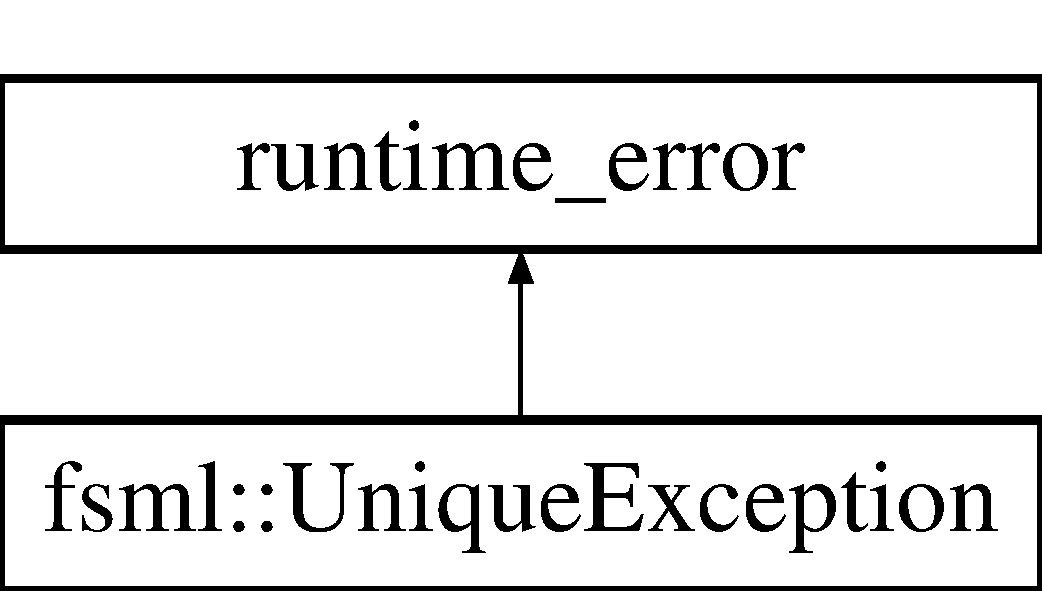
\includegraphics[height=2.000000cm]{structfsml_1_1UniqueException}
\end{center}
\end{figure}
\subsection*{Public Member Functions}
\begin{DoxyCompactItemize}
\item 
\hypertarget{structfsml_1_1UniqueException_a14fc471605daa57d638a35756fa66901}{{\bfseries Unique\-Exception} (const std\-::string \&state)}\label{structfsml_1_1UniqueException_a14fc471605daa57d638a35756fa66901}

\end{DoxyCompactItemize}


The documentation for this struct was generated from the following files\-:\begin{DoxyCompactItemize}
\item 
include/fsml/Exceptions.\-hpp\item 
src/fsml/Exceptions.\-cpp\end{DoxyCompactItemize}

\addcontentsline{toc}{part}{Index}
\printindex
\end{document}
